% =====================================================================
%  PORTADA
%  Página 1: imagen de portada a página completa (img/portada.pdf)
%  Página 2: en blanco
%  Página 3: portada interior con título, autor, tutor y logos
% =====================================================================

% Imagen de fondo solo en la primera página
\AddToShipoutPictureBG*{%
	\put(0,0){%
		\parbox[b][\paperheight]{\paperwidth}{%
			\vfill
			\centering
			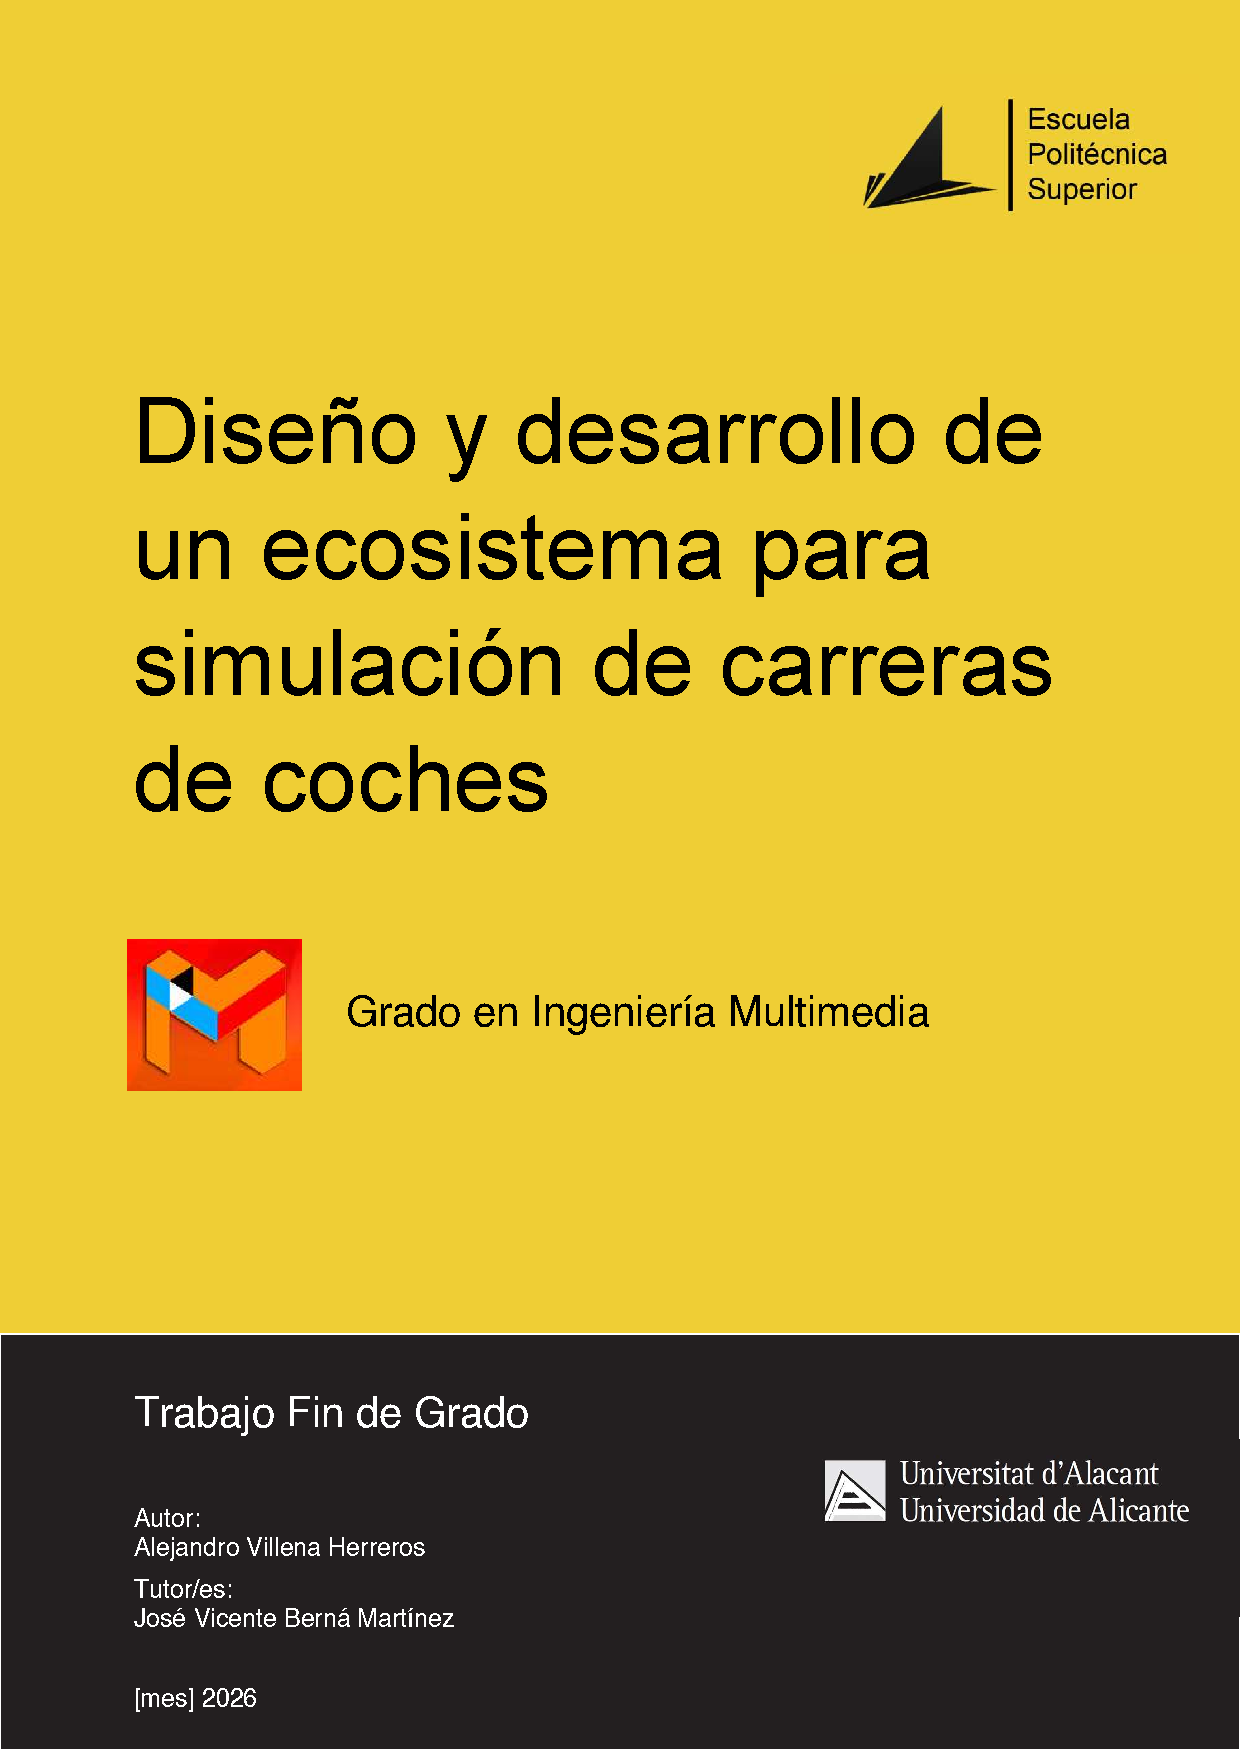
\includegraphics[width=\paperwidth]{img/portada.pdf}
			\vfill
		}%
	}%
}

% Página de la portada (con la imagen de fondo)
\thispagestyle{empty}
\mbox{}

% Hoja en blanco
\newpage
\thispagestyle{empty}
\mbox{}

% Portada interior
\begin{titlepage}
	\centering
	\vspace*{1.5cm}

	{\LARGE \textbf{Diseño y desarrollo de un ecosistema para simulación de carreras de coches}}\\[0.3cm]

	\vspace{0.3cm}
	\rule{\linewidth}{0.8pt}

	\vspace{2cm}

	\textbf{Autor:}\\[0.2cm]
	Alejandro Villena Herreros

	\vspace{1.5cm}

	\textbf{Tutor:}\\[0.2cm]
	José Vicente Berná Martínez \\
	Departamento de Tecnología Informática y Computación

	\vfill

	
\includegraphics[height=1.8cm]{img/logo_eps.png}
	\hspace{1.5cm}
	
\includegraphics[height=1.8cm]{img/logo_ua.jpg}

	\vspace{1cm}

	\textbf{ALICANTE, mes 2026}

\end{titlepage}

% Hoja en blanco tras la portada
\newpage
\thispagestyle{empty}
\mbox{}
